% Template for a Computer Science Tripos Part II project dissertation
\documentclass[12pt,a4paper,twoside, openright, hidelinks]{report}
\usepackage[pdfborder={0 0 0}]{hyperref}
\urlstyle{same}
\usepackage[margin=25mm]{geometry} 
\usepackage{graphicx} % allows inclusion of PDF, PNG and JPG images
\usepackage{verbatim}
\usepackage{docmute} % only needed to allow inclusion of proposal.tex

\usepackage{bookmark}
\usepackage{amsmath}
\usepackage{parskip}
\usepackage{enumitem}

\usepackage{xcolor}
\usepackage[multiple]{footmisc}

\raggedbottom                           % try to avoid widows and orphans
\sloppy
\clubpenalty1000%
\widowpenalty1000%

\renewcommand{\baselinestretch}{1.1}    % adjust line spacing to make
                                        % more readable

\begin{document}
\bibliographystyle{plain}
%%%%%%%%%%%%%%%%%%%%%%%%%%%%%%%%%%%%%%%%%%%%%%%%%%%%%%%%%%%%%%%%%%%%%%%%
% Title
\pagestyle{empty}

\rightline{\large{Kamilė Stankevičiūtė}}

\vspace*{60mm}
\begin{center}
\LARGE
\textbf{Graph neural networks for age prediction from neuroimaging data} \\[5mm]
\large
Computer Science Tripos -- Part II \\[5mm]
Gonville \& Caius College \\[5mm]
\today  % today's date
\end{center}

%%%%%%%%%%%%%%%%%%%%%%%%%%%%%%%%%%%%%%%%%%%%%%%%%%%%%%%%%%%%%%%%%%%%%%%%%%%%%%
% Proforma, table of contents and list of figures

\pagestyle{plain}

\chapter*{Proforma}

\begin{tabular}{ll}
Name:               & Kamilė Stankevičiūtė                     \\
College:            & Gonville \& Caius College                     \\
Project title:      & Graph neural networks for age prediction from neuroimaging data \\
Examination:        & Computer Science Tripos -- Part II 2020 \\
Word count:         & ?\footnotemark[1] \\
Lines of code:      & ?  \\
Project originator: & Mr Tiago Azevedo                        \\
Supervisors:        & Mr Tiago Azevedo, Mr Alexander Campbell \\ 
\end{tabular}
\footnotetext[1]{Counted using the \LaTeX\ Utilities extension in Visual Studio Code.}
\stepcounter{footnote}



\section*{Original Aims of the Project}

To write a demonstration dissertation\footnote{A normal footnote without the
complication of being in a table.} using \LaTeX\ to save
student's time when writing their own dissertations. The dissertation
should illustrate how to use the more common \LaTeX\ constructs. It
should include pictures and diagrams to show how these can be
incorporated into the dissertation.  It should contain the entire
\LaTeX\ source of the dissertation and the makefile.  It should
explain how to construct an MSDOS disk of the dissertation in
Postscript format that can be used by the book shop for printing, and,
finally, it should have the prescribed layout and format of a diploma
dissertation.


\section*{Work Completed}

All that has been completed appears in this dissertation.

\section*{Special Difficulties}

None.
 
\newpage
\section*{Declaration}

I, Kamilė Stankevičiūtė of Gonville \& Caius College, being a candidate for Part II of the Computer Science Tripos, hereby declare that this dissertation and the work described in it are my own work, unaided except as may be specified below, and that the dissertation does not contain material that has already been used to any substantial extent for a comparable purpose.

\bigskip
\leftline{Signed \textit{Kamilė Stankevičiūtė}}

\medskip
\leftline{Date \today}

\tableofcontents

\listoffigures

\newpage
\section*{Acknowledgements}

This document owes much to an earlier version written by Simon Moore
\cite{Moore95}.  His help, encouragement and advice was greatly 
appreciated.

%%%%%%%%%%%%%%%%%%%%%%%%%%%%%%%%%%%%%%%%%%%%%%%%%%%%%%%%%%%%%%%%%%%%%%%
% now for the chapters

\pagestyle{headings}

\chapter{Introduction}

\section{Overview of the files}

This document consists of the following files:

\begin{itemize}
\item \texttt{makefile} --- The makefile for the dissertation and
                         Project Proposal
\item \texttt{diss.tex} --- The dissertation
\item \texttt{proposal.tex}  --- The project proposal 
\item \texttt{figs} -- A directory containing diagrams and pictures
\item \texttt{refs.bib} --- The bibliography database
\end{itemize}

\section{Building the document}

This document was produced using \LaTeXe which is based upon
\LaTeX\cite{Lamport86}.  To build the document you first need to
generate \texttt{diss.aux} which, amongst other things, contains the
references used.  This if done by executing the command:

\texttt{pdflatex diss}

\noindent
Then the bibliography can be generated from \texttt{refs.bib} using:

\texttt{bibtex diss}

\noindent
Finally, to ensure all the page numbering is correct run \texttt{pdflatex}
on \texttt{diss.tex} until the \texttt{.aux} files do not change.  This
usually takes 2 more runs.

\subsection{The makefile}

To simplify the calls to \texttt{pdflatex} and \texttt{bibtex}, 
a makefile has been provided, see Appendix~\ref{makefile}. 
It provides the following facilities:

\begin{description}

\item\texttt{make} \\
 Display help information.

\item\texttt{make proposal.pdf} \\
 Format the proposal document as a PDF.

\item\texttt{make view-proposal} \\
 Run \texttt{make proposal.pdf} and then display it with a Linux PDF viewer
 (preferably ``okular'', if that is not available fall back to ``evince'').

\item\texttt{make diss.pdf} \\
 Format the dissertation document as a PDF.

\item\texttt{make count} \\
Display an estimate of the word count.

\item\texttt{make all} \\
Construct \texttt{proposal.pdf} and \texttt{diss.pdf}.

\item\texttt{make pub} \\ Make \texttt{diss.pdf}
and place it in my \texttt{public\_html} directory.

\item\texttt{make clean} \\ Delete all intermediate files except the
source files and the resulting PDFs. All these deleted files can
be reconstructed by typing \texttt{make all}.

\end{description}


\section{Counting words}

An approximate word count of the body of the dissertation may be
obtained using:

\texttt{wc diss.tex}

\noindent
Alternatively, try something like:

\verb/detex diss.tex | tr -cd '0-9A-Z a-z\n' | wc -w/


\chapter{Preparation}

This chapter is empty!


\chapter{Implementation}

\section{Verbatim text}

Verbatim text can be included using \verb|\begin{verbatim}| and
\verb|\end{verbatim}|. I normally use a slightly smaller font and
often squeeze the lines a little closer together, as in:

{\renewcommand{\baselinestretch}{0.8}\small
\begin{verbatim}
GET "libhdr"
 
GLOBAL { count:200; all  }
 
LET try(ld, row, rd) BE TEST row=all
                        THEN count := count + 1
                        ELSE { LET poss = all & ~(ld | row | rd)
                               UNTIL poss=0 DO
                               { LET p = poss & -poss
                                 poss := poss - p
                                 try(ld+p << 1, row+p, rd+p >> 1)
                               }
                             }
LET start() = VALOF
{ all := 1
  FOR i = 1 TO 12 DO
  { count := 0
    try(0, 0, 0)
    writef("Number of solutions to %i2-queens is %i5*n", i, count)
    all := 2*all + 1
  }
  RESULTIS 0
}
\end{verbatim}
}

\section{Tables}

\begin{samepage}
Here is a simple example\footnote{A footnote} of a table.

\begin{center}
\begin{tabular}{l|c|r}
Left      & Centred & Right \\
Justified &         & Justified \\[3mm]
%\hline\\%[-2mm]
First     & A       & XXX \\
Second    & AA      & XX  \\
Last      & AAA     & X   \\
\end{tabular}
\end{center}

\noindent
There is another example table in the proforma.
\end{samepage}

\section{Simple diagrams}

Simple diagrams can be written directly in \LaTeX.  For example, see
figure~\ref{latexpic1} on page~\pageref{latexpic1} and see
figure~\ref{latexpic2} on page~\pageref{latexpic2}.

\begin{figure}
\setlength{\unitlength}{1mm}
\begin{center}
\begin{picture}(125,100)
\put(0,80){\framebox(50,10){AAA}}
\put(0,60){\framebox(50,10){BBB}}
\put(0,40){\framebox(50,10){CCC}}
\put(0,20){\framebox(50,10){DDD}}
\put(0,00){\framebox(50,10){EEE}}

\put(75,80){\framebox(50,10){XXX}}
\put(75,60){\framebox(50,10){YYY}}
\put(75,40){\framebox(50,10){ZZZ}}

\put(25,80){\vector(0,-1){10}}
\put(25,60){\vector(0,-1){10}}
\put(25,50){\vector(0,1){10}}
\put(25,40){\vector(0,-1){10}}
\put(25,20){\vector(0,-1){10}}

\put(100,80){\vector(0,-1){10}}
\put(100,70){\vector(0,1){10}}
\put(100,60){\vector(0,-1){10}}
\put(100,50){\vector(0,1){10}}

\put(50,65){\vector(1,0){25}}
\put(75,65){\vector(-1,0){25}}
\end{picture}
\end{center}
\caption{A picture composed of boxes and vectors.}
\label{latexpic1}
\end{figure}

\begin{figure}
\setlength{\unitlength}{1mm}
\begin{center}

\begin{picture}(100,70)
\put(47,65){\circle{10}}
\put(45,64){abc}

\put(37,45){\circle{10}}
\put(37,51){\line(1,1){7}}
\put(35,44){def}

\put(57,25){\circle{10}}
\put(57,31){\line(-1,3){9}}
\put(57,31){\line(-3,2){15}}
\put(55,24){ghi}

\put(32,0){\framebox(10,10){A}}
\put(52,0){\framebox(10,10){B}}
\put(37,12){\line(0,1){26}}
\put(37,12){\line(2,1){15}}
\put(57,12){\line(0,2){6}}
\end{picture}

\end{center}
\caption{A diagram composed of circles, lines and boxes.}
\label{latexpic2}
\end{figure}



\section{Adding more complicated graphics}

The use of \LaTeX\ format can be tedious and it is often better to use
encapsulated postscript (EPS) or PDF to represent complicated graphics.
Figure~\ref{epsfig} and~\ref{xfig} on page \pageref{xfig} are
examples. The second figure was drawn using \texttt{xfig} and exported in
{\tt.eps} format. This is my recommended way of drawing all diagrams.


\begin{figure}[tbh]
\centerline{\includegraphics{figs/cuarms.pdf}}
\caption{Example figure using encapsulated postscript}
\label{epsfig}
\end{figure}

\begin{figure}[tbh]
\vspace{4in}
\caption{Example figure where a picture can be pasted in}
\label{pastedfig}
\end{figure}


\begin{figure}[tbh]
\centerline{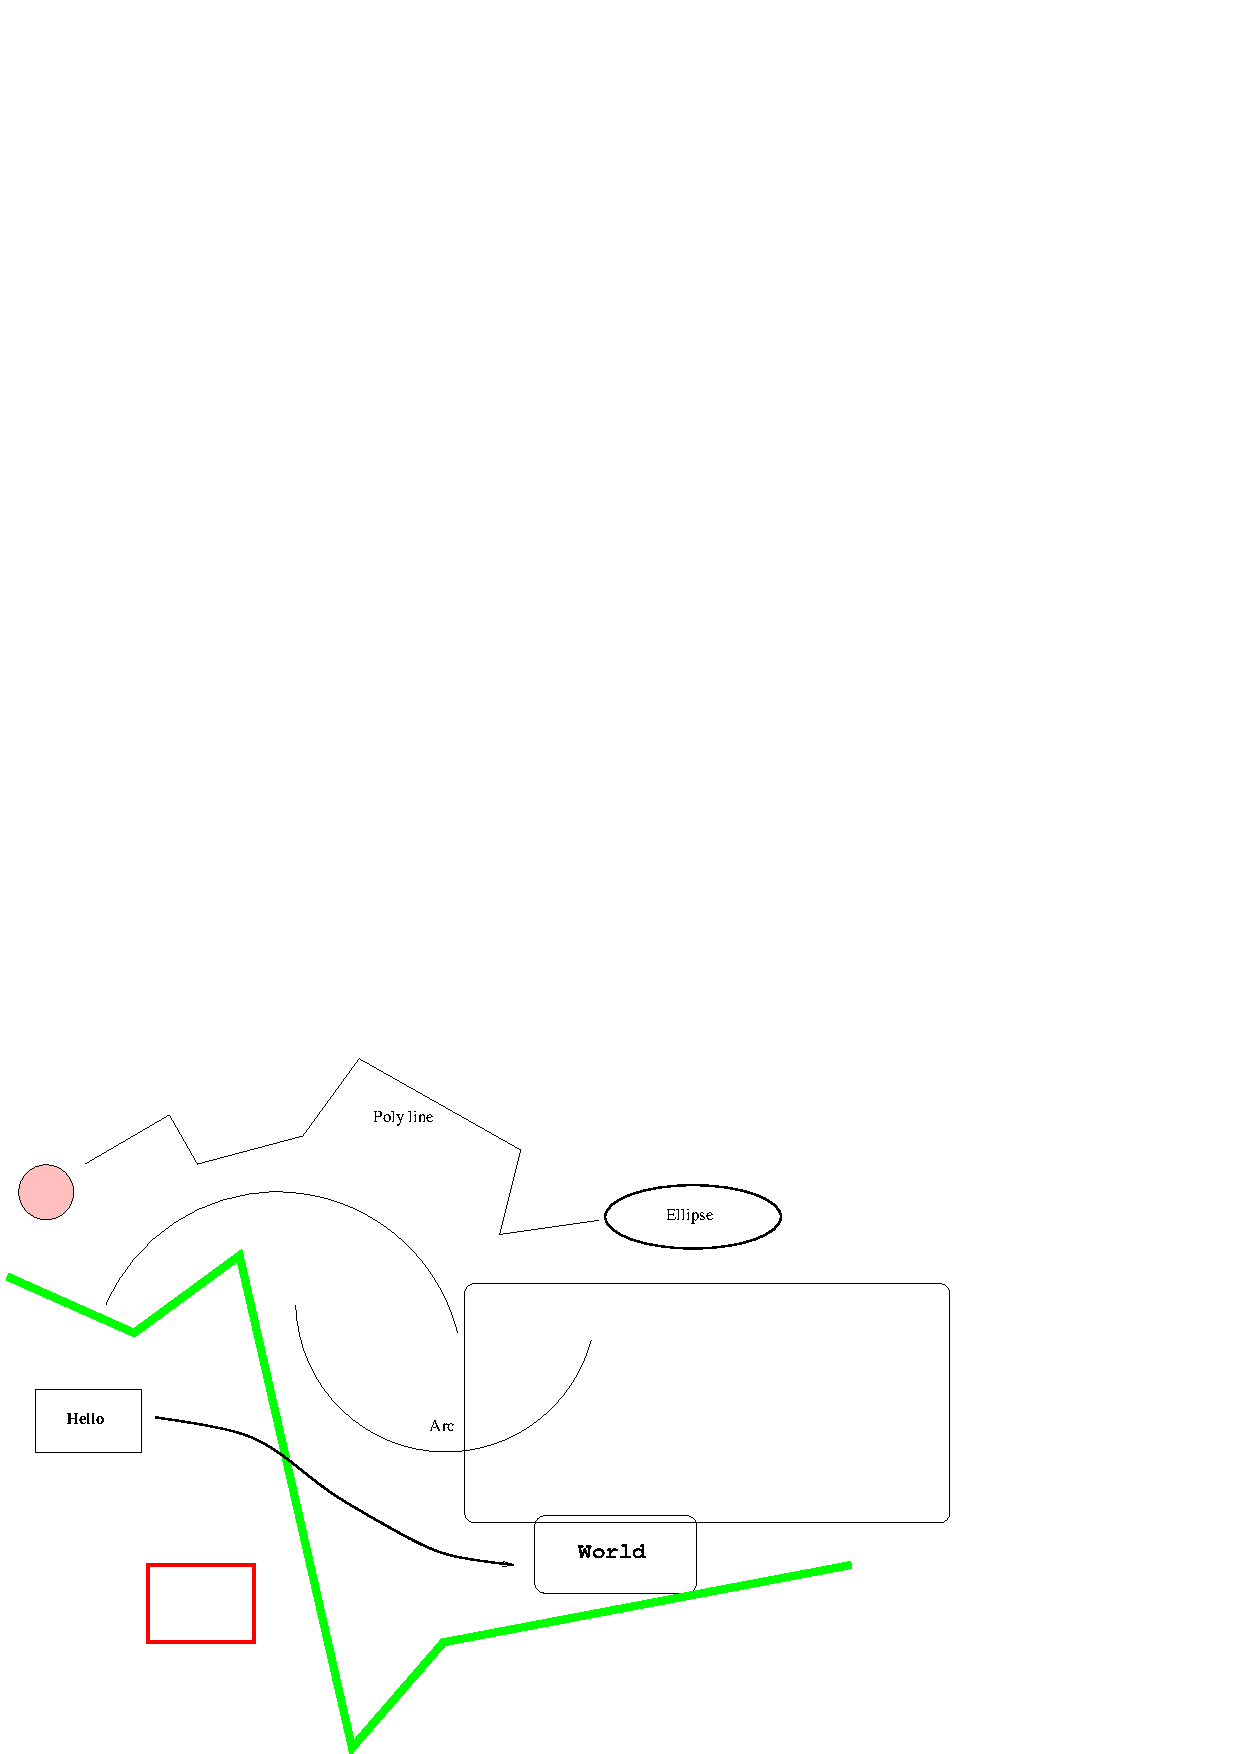
\includegraphics{figs/diagram.pdf}}
\caption{Example diagram drawn using \texttt{xfig}}
\label{xfig}
\end{figure}


\chapter{Evaluation}

\section{Printing and binding}

Use a ``duplex'' laser printer that can print on both sides to print
two copies of your dissertation. Then bind them, for example using the
comb binder in the Computer Laboratory Library.

\section{Further information}

See the Unix Tools notes at

\url{http://www.cl.cam.ac.uk/teaching/current-1/UnixTools/materials.html}


\chapter{Conclusion}

I hope that this rough guide to writing a dissertation is \LaTeX\ has
been helpful and saved you time.


%%%%%%%%%%%%%%%%%%%%%%%%%%%%%%%%%%%%%%%%%%%%%%%%%%%%%%%%%%%%%%%%%%%%%
% the bibliography
\addcontentsline{toc}{chapter}{Bibliography}
\bibliography{refs}

%%%%%%%%%%%%%%%%%%%%%%%%%%%%%%%%%%%%%%%%%%%%%%%%%%%%%%%%%%%%%%%%%%%%%
% the appendices
\appendix

\chapter{Latex source}

\section{diss.tex}
{\scriptsize\verbatiminput{diss.tex}}

\section{proposal.tex}
{\scriptsize\verbatiminput{proposal.tex}}

% \chapter{Makefile}

% \section{makefile}\label{makefile}
% {\scriptsize\verbatiminput{makefile.txt}}

\section{refs.bib}
{\scriptsize\verbatiminput{refs.bib}}

\section{references.bib}
{\scriptsize\verbatiminput{references.bib}}

\chapter{Project Proposal}

% \documentclass[12pt,a4paper,twoside, hidelinks]{article}
% \usepackage{bookmark}
% \usepackage{amsmath}
% \usepackage{parskip}
% \usepackage{enumitem}
% \usepackage{hyperref}
% \urlstyle{same}
% \usepackage{xcolor}
% \usepackage[multiple]{footmisc}
% \usepackage[margin=25mm]{geometry}
% % \usepackage[backend=biber, maxnames=4]{biblatex}
% % \addbibresource{stankeviciute-proposal.bib}

% \begin{document}
\chapter{Project proposal}
\label{chapter:project-proposal}

\begin{center}
\Large
Computer Science Tripos -- Part II -- Project Proposal\\[4mm]
\LARGE
Graph neural networks for age prediction from neuroimaging data \\[4mm]

\large
2419E

% \today % October 2019
\end{center}

\vspace{5mm}
\textbf{Project Originator:} Tiago Azevedo

\textbf{Project Supervisors:} Tiago Azevedo, Alexander Campbell, Prof Pietro Liò

\textbf{Project Overseers:} Prof Jon~Crowcroft, Dr Thomas~Sauerwald

% Main document

\section*{Introduction}
% The problem to be addressed.

% [Tiago] Why NNs and not something else? You probably want one sentence of motivation saying they have been very successful in other fields, and then one sentence that as a consequence they might help physicians.
% \textit{...Neural networks provide the opportunity to capture the similarities between patients and trends which might help physicians to understand the mechanisms of the disease and in turn find more effective treatments...}

A graph neural network (GNN) is a type of a neural network that operates on graph inputs and is used for tasks like node classification, link prediction and clustering (geometric deep learning). GNNs have recently become popular and proved successful in a broad range of real-world applications, such as text and image classification, knowledge graphs, and interaction modelling in physical and biological systems. \cite{zhou2018gnn}

One domain where graphs offer a natural representation is social networks and \textit{populations}, with nodes representing individuals (their features and labels), and edges corresponding to associations between individuals according to some heuristic or a formally defined similarity metric. The reason why such graph representation is considered to be useful in the geometric deep learning context is that the network can make use of both the individual features (node feature vectors) and the overall trends in the population through pairwise similarities (graph edges), \cite{parisot2017spectral} inferring the label of an individual node both from the node itself and from its neighbourhood.
% The graph structure is also helpful when incorporating multiple modalities of data, which is often the case for medical records containing, for example, imaging and non-imaging data. 

\section*{Project description}
This project was inspired by Parisot et al.'s \cite{parisot2017spectral, parisot2018disease} state-of-the-art application of a type of a GNN called Graph Convolutional Network (GCN) to the population graphs of healthy controls and patients with neurological or neurodegenerative disorders. In these papers, the GCN (adapted from Kipf and Welling \cite{kipf2017semi}) was used in a semi-supervised manner for two classification tasks: 1) prediction of autism spectrum disorder (ASD) from the ABIDE dataset and 2) prediction of a progressive form of Mild Cognitive Impairment (MCI) that develops into Alzheimer's disease (AD) from the ADNI dataset.

Moreover, a recent paper by Kaufmann et al. \cite{kaufmann2019} has linked the incidence of common brain disorders, including ASD, MCI, and AD as well as others, to the deviation between chronological and biological brain ageing. These results suggest that being able to estimate the subject's age from the neuroimaging data may be important in understanding the mechanisms of those disorders and helping physicians to find more effective treatments.

The aim of this project will therefore be to adapt the population graph approach of Parisot et al. \cite{parisot2017spectral, parisot2018disease} to a regression task on the UK Biobank dataset, predicting the subject's age based on neuroimaging data, and comparing it to another successful geometric deep learning architecture such as the Graph Attention Network. \cite{velickovic2018graph} The performance of the networks will be evaluated on the standard metrics, e.g. the coefficient of determination~$r^2$.

\section*{Starting point}
% Describe existing state of the art, previous work in this area,
%   libraries and databases to be used. Describe the state of any
%   existing codebase that is to be built on.

The source code for the implementation of Kipf and Welling's \cite{kipf2017semi} GCNs and Parisot et al.'s \cite{parisot2017spectral, parisot2018disease} first classification task is publicly available online.\footnote{\url{https://github.com/tkipf/gcn}}\footnote{\url{https://github.com/parisots/population-gcn}}

I will be using PyTorch for this project because of its support for machine learning on structured graph data. In particular, PyTorch Geometric (PyG)\footnote{\url{https://github.com/rusty1s/pytorch_geometric}} – a geometric deep learning extension library – will make the implementation, iteration and extensions to the model more flexible in addition to performance improvements and simplified APIs.
% making the final library more accessible and extensible, contributing to the open-source community

I have experience with the basics of TensorFlow\footnote{Five-course Deep Learning specialisation by deeplearning.ai on Coursera}\footnote{Google's Machine Learning Crash Course and follow-up courses.} and no experience with PyTorch or graph neural networks. I have attended or will study (possibly in advance) the CST courses related to the subject of this project, such as IA Machine Learning and Real-World Data, IB Artificial Intelligence, II Data Science, II Bioinformatics, and II Machine Learning and Bayesian Inference.

\subsection*{Dataset}

I will be using the data from the UK Biobank, kindly preprocessed and provided by Dr~Richard Bethlehem of the Department of Psychiatry.

The UK Biobank is a large dataset containing comprehensive phenotypic, genetic, MRI and other data from the total of over 500,000 participants.\footnote{\url{https://www.ukbiobank.ac.uk/participants/}} In this project, I will be using the subset of this dataset with only those subjects who had the neuroimaging data collected and preprocessed (approximately 20,000 participants). This includes both structural (T1, T2 FLAIR) and functional (resting state fMRI) data, preprocessed with the standard UK Biobank pipelines\footnote{\url{https://biobank.ctsu.ox.ac.uk/crystal/crystal/docs/brain_mri.pdf}} and additionally denoised and parcellated (in several common parcellations) by Dr Bethlehem. 
% I am likely to be using the correlation matrices and raw parcellated time series for functional and features like coritical thickness for structural data.

\section*{Work to be done}
\label{section:work}

% [Tiago] bullet points should start with the same sentence structure

% Describe the technical work.
The following are lists of explicit deliverables to be implemented.

\textbf{Graph neural network framework}
\begin{enumerate}[label=G\arabic*.]
  \item The data is preprocessed into features and is ready for analysis. % [Tiago] "data cleaned and is ready for analysis" 
  \item Definition of the similarity metric to be used in connecting the graph. The graph is connected based on that similarity metric to be processed by graph neural networks.
  \item Implementation of Kipf's GCN \cite{kipf2017semi} for the age regression task.
  % [Tiago] GAT originally doesn't allow for weighted edges. You probably want to say GAT because of interesting results in previous literature. Thus, you can probably divide this point: (1) implementation of another graph NN layer, (2) Include weights (in theory you can even edit the message passing mechanism in GCN to multiply by the weights, just like you are suggesting for GAT) 
  \item Implementation of the Graph Attention Network for comparing its performance to the Graph Convolutional Network.
  % [Tiago] What exactly would you be testing points? Eg. what a unit test would consist of?
  % [Tiago] I just recalled that one thing we discussed could be how it handles missing data (eg. a certain percentage without some data), which could create an interesting view on robustness and semi-supervised learning. Maybe this could go to extension (or "personal" extension in case you have time and you can say you had one more extension than initially planned)
\end{enumerate}

\textbf{Evaluation framework}

\begin{enumerate}[label=E\arabic*.]
  \item  Comparison of the alternative graph neural network models using the coefficient of determination $r^2$.
\end{enumerate}

\section*{Success criteria}
% Describe what you expect to be able to demonstrate at the
% end of the project and how you are going to evaluate your achievement.
The project will be successful if the following items will have been implemented.
\begin{enumerate}[label=SC\arabic*.]
  \item Representation of the UK Biobank data as a population graph with nodes representing the individuals and edges representing associations between them based on pairwise similarity.
  \item The Graph Convolutional Network for age regression on the population graph.
  \item The Graph Attention Network for the same task.
  \item The evaluation framework for comparing the performance of the two graph neural networks.
\end{enumerate}

\section*{Evaluation of the project}
The performance of the graph neural networks will be measured across several metrics. The main metric to evaluate a regression task, in contrast the classification in Parisot et al. \cite{parisot2018disease}, is the coefficient of determination~$r^2$. 

\section*{Possible extensions}
% Potential further envisaged evaluation metrics or extensions.
\begin{enumerate}[label=PE\arabic*.]
  \item An additional metric that could be used to evaluate the performance of the networks is \textit{robustness} to missing or noisy data. Robustness, which could be defined as \textit{the rate at which the predictive power drops as more information is removed from the nodes}, would reveal how important is the neighbourhood (edge) information for accurate predictions compared to the node features only.
  \item Implement spectral filter computation with \textit{Cayley polynomials} instead of using Chebyshev polynomials. Cayley polynomials have been introduced in a paper by Levie et al. \cite{levie2017cayleynets} and were mentioned in Parisot et al. \cite{parisot2018disease} as a possible improvement.
  \item The main implementation of the graph neural network relies on manually handcrafted features from preprocessed brain imaging data. Time permitting, an extension could be to create a package that can be used after any standard neuroimaging preprocessing pipeline (e.g. with results in BIDS\footnote{\url{https://bids.neuroimaging.io}} format) to extract these features, and possibly improve upon as well as create new ones. This would make execution of the model more efficient, robust and generalisable.
  \item Implement weighted edges in the Graph Convolutional Network and Graph Attention Network, as the main implementations will have binary edges.
  % \item Implement a \textit{custom similarity metric}. The metrics used in the work by Parisot et al. \cite{parisot2018disease} were defined arbitrarily by the authors based on very few features. Learning a different similarity metric based on more combinations of features could possibly result in a better performance of the classifier.

\end{enumerate}


\section*{Timetable and milestones}
\label{section:timetable}

% A work plan of perhaps ten or so two-week work-packages,
% as well as milestones to be achieved along the way. Provide a
% target date for each milestone.

% [Tiago] you can specify which parts of the work you intend to implement in each 2-week time frame. This will help you having a better idea of how you are keeping up/behind.

%  (01/10/2019 – 16/10/2019)
\textbf{Michaelmas weeks 0–1}
\begin{itemize}
  \item Work on project proposal.
\end{itemize}

\textbf{Milestones.} Submit Phase 1 report by 14/10/2019. Submit draft proposal by 18/10/2019.

% (17/10/2019 – 06/11/2019)
\textbf{Michaelmas weeks 2–4}
\begin{itemize}
  \item Get access to the UK Biobank data and get familiar with its features.
  \item Define a possible graph similarity metric.
\end{itemize}

\textbf{Milestones.} Submit final project proposal by 25/10/2019.

% (07/11/2019 – 20/11/2019)
\textbf{Michaelmas weeks 5–6}
\begin{itemize}
  \item Write code for connecting the nodes based on a similarity metric.
  \item Connect the nodes (with their features) into a graph.
  \item Start working on the implementation of the Graph Convolutional Network (e.g. define loss and random label removal for semi-supervised training, start implementing the layers).
\end{itemize}

% (21/11/2019 – 04/12/2019)
\textbf{Michaelmas weeks 7–8} 
\begin{itemize}
  \item Work on the implementation of layers for the Graph Convolutional Network. Compute the general performance metrics.
  \item Start working on Graph Attention Network implementation for the same task.
\end{itemize}

\textbf{Michaelmas vacation}
\begin{itemize}
  \item Continue working on and finish the neural network implementations, compute performance metrics.
  \item Work on graph neural network evaluation: implement the robustness measurement framework.
  \item Measure the robustness of the neural networks.
  \item Start writing the dissertation and the project progress report.
\end{itemize}

\textbf{Milestones.} Complete the implementation of the main part of the project.

% (16/01/2020 – 29/01/2020)
\textbf{Lent weeks 0–2}
\begin{itemize}
  \item Finish the progress report, prepare for the presentation.
  \item Implement Cayley polynomials.
  \item Start working on the data preprocessing pipeline.
\end{itemize}
 
\textbf{Milestones.} Submit progress report by 31/01/2020.

% (30/01/2020 – 19/02/2020)
\textbf{Lent weeks 3–5}
\begin{itemize}
  \item Continue implementing the data preprocessing pipeline.
  \item Start working on the implementation of weighted edges.
\end{itemize}


% (20/02/2020 – 11/03/2020)
\textbf{Lent weeks 6–8}
\begin{itemize}
  \item Finish implementing the data preprocessing pipeline.
  \item Finish implementing the weighted edges.
  \item Continue working on the dissertation write-up.
\end{itemize}

\textbf{Easter vacation}
\begin{itemize}
  \item Complete the dissertation draft and send it for review.
  \item Edit the draft based on the feedback received.
\end{itemize}

\textbf{Milestones.} Send out the complete draft for review by 27/03/2020. Submit dissertation early by 20/04/2020.

% (24/04/2020 – 06/05/2020)
\textbf{Easter weeks 0–2}

 Time reserved for any unexpected issues.

 \section*{Resource declaration}

 For this project I will be using my personal MacBook Pro (2019, with 1.4 GHz Quad-Core Intel Core i5 processor and 8GB of RAM). Training the model will require the use of GPUs provided by the Computational Biology Group (as confirmed by Prof Pietro Liò). To prevent any loss of data, both the source code and the \LaTeX\ source will be stored on my machine, private GitHub repositories, and Google Drive, as well as regularly backed up on an external HDD.

% \medskip 
% \printbibliography


\end{document}
